\documentclass[12pt]{article}
\usepackage[letterpaper,top=2.54cm,bottom=2.54cm,left=2.54cm,right=2.54cm,marginparwidth=1.75cm]{geometry}
%% Language and font encodings
\usepackage[english]{babel}
\usepackage[utf8x]{inputenc}
\usepackage[T1]{fontenc}
\usepackage{graphicx}
\usepackage{subcaption}
\usepackage{mwe}
\usepackage{float}
\usepackage{amsmath}
\usepackage{multicol}
\usepackage[colorinlistoftodos]{todonotes}
\usepackage[colorlinks=true, allcolors=blue]{hyperref}
\usepackage{listings}
\usepackage{mathptmx}
\usepackage{color}
\usepackage{amsmath}
\usepackage{amssymb}
\usepackage{epstopdf}
\usepackage{inputenc}
\usepackage{geometry}
\usepackage{color}
\usepackage[nottoc]{tocbibind}
\usepackage{natbib}
\usepackage{courier}
\usepackage{algorithm}
\usepackage[noend]{algpseudocode}
\usepackage{qtree}
\usepackage{forest}

\makeatletter
\def\BState{\State\hskip-\ALG@thistlm}
\makeatother

%% Matlab
\definecolor{mygreen}{RGB}{28,172,0} % color values Red, Green, Blue
\definecolor{mylilas}{RGB}{170,55,241}

\lstset{language=Matlab,%
    basicstyle=\scriptsize\ttfamily,
    breaklines=true,%
    morekeywords={matlab2tikz},
    keywordstyle=\color{blue},%
    morekeywords=[2]{1}, keywordstyle=[2]{\color{black}},
    identifierstyle=\color{black},%
    stringstyle=\color{mylilas},
    commentstyle=\color{mygreen},%
    showstringspaces=false,%without this there will be a symbol in the places where there is a space
    numbers=left,%
    numberstyle={\tiny \color{black}},% size of the numbers
    numbersep=9pt, % this defines how far the numbers are from the text
    emph=[1]{for,end,break},emphstyle=[1]\color{red}, %some words to emphasise
    emph=[2]{word1,word2}, emphstyle=[2]{style},    
}


\begin{document}
\begin{titlepage}
	\centering
	{\scshape\LARGE Columbia University \par}
	\vspace{1cm}
	{\scshape MECE 4510 Evolutionary Computation and Design Automation\par}
	\vspace{1.5cm}
	{\huge\bfseries Symbolic Regression\par}
	\vspace{2cm}
	{\Large\itshape Hanwen Zhao\par}
	{UNI: hz2547\par}
	\vfill
	supervised by\par
	Dr.~Hod \textsc{Lipson}
	\vfill
	Grace Hours Used: 53\\
	Grace Hours Remaining: 43 \\
	\vspace{2cm}
% Bottom of the page
	{\large \today\par}
\end{titlepage}

\newpage
\section{Result Summary}
\begin{table}[!h]
\footnotesize
	\begin{center}
		\begin{tabular}{|c|c|c|}
			\hline
			\multicolumn{3}{|c|}{Result Table}\\
			\hline
			Method & Evaluation Number & Best Error (MAE)\\
			\hline
			Random Search & 300000 & 0.0847\\
			\hline
			Hill Climber & 300000 & 0.0863\\
			\hline
			GP (Conventional Selection) & 14000 & 0.00002537\\
			\hline
			GP (Conventional Selection) with Larger Population & 43000 & 0.00002537\\
			\hline
			GP (Deterministic Crowding) & 129000 & 0.00002537\\
			\hline
		\end{tabular}
	\end{center}
\end{table}

\begin{figure}[H]
	\centering
	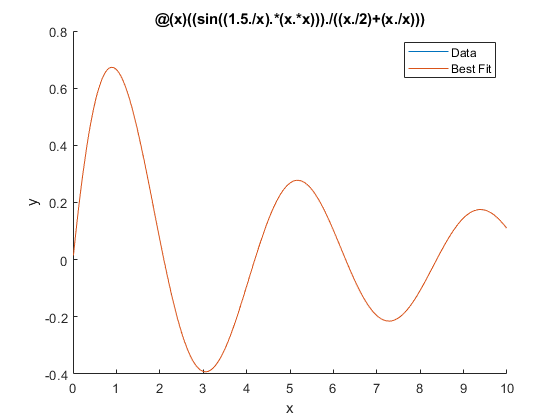
\includegraphics[width=0.75\textwidth]{bestFit}
	\caption[]%
	{{\small Performance Plot}}    
\end{figure}

After simplification, the function can be expressed as:
\begin{equation}
f(x) = sin(1.5x)/(0.5x+1)
\end{equation}

\newpage
\section{Methods}
For this homework, we have been asked to use genetic programming to perform symbolic regression. Our goal is to find the symbolic algebraic expression in the form of $y=f(x)$ that best fits a set of given 1000 $(x,y)$ points. Assume the symbolic regression only uses algebraic operators: $x,\ -,\ *,\ /$, $sine\ and\ cosine$, and real constants(in the range $\pm10$), and the variable x.
\subsection{Representation}
The key part of genetic programming is to covert the program into a high level tree structure compare to genetic programming which the program was converted into simpler chromosome type. The tree structure is more powerful in terms of computer programming since trees can be easy evaluated in a recursive manner.
For example, a function can be represented as a tree structure as following:\\
\begin{center}
\begin{forest}
[$+$
	[$-$
		[2.2]
		[$\div$
			[$X$]
			[$11$]
		]
	]
	[$*$
		[$7$]
		[$cos$
			[$X$]
		]
	]
]
\end{forest}
\end{center}
can represent the equation
\begin{equation}
(2.2-\frac{x}{11})+(7*cos(x))
\end{equation}
For this assignment, we assume the maximum depth of the tree structure is less and equal than 5.
\subsection{Random Search}
Once we have our representation setup, the random search algorithm is straight forward. For each evaluation of the random search algorithm, a function tree is generated with random depth  from two to five. The random search is the baseline for performance comparison between the hill climber algorithm and our genetic programmings.
\subsection{Random Hill Climber}
A Random Hill Climber is basically a random search with simple decision making capability. Between each evaluation, the mutation process is applied to the function. During the mutation process, it will randomly select a valid mutation point, generate a new sub-tree and replace into new function tree. In my implementation, the probability decide whether it always go to a better solution or not. Sometime go to a worse solution can avoid hill climber stuck at the local maximum. 


\subsection{Genetic Programming with Variations}
Similar to Evolutionary Algorithm, we can implement following types of operators into the Genetic Programming: selection, crossover, and mutation. For variation, Deterministic Crowding and different size of population was applied during my implementation. Here are some details about the techniques I used in my implementation:\\
\vspace{-5mm}
\begin{itemize}
	\setlength\itemsep{0.1em}
	\item Selection: For conventional selection Genetic Programming, during each generation, a default of 50\% parents will be selected to generate 50 offsprings.
	\item Crossover: The crossover was applied into both conventional selection method and deterministic crowding method. The algorithm will first choose two valid crossover node from each parent and switch the subtrees between two parents in order to generate two offSprings.
	\item Mutation: During the mutation process, the algorithm will first randomly pick a valid node for mutation, then generate a new tree based on the depth of the mutation node.
	\item Deterministic Crowding: In order to maintain the diversity for genetic programming, we need some methods to maintain useful diversity for genetic programming to work better. Crowding is one of the popular method, it only replace individuals that are similar. More specific, deterministic crowding compare the similarity between two parents and two offsrpings, replace the one has higher similarity.\\
	
\begin{algorithm}[H]
\caption{Deterministic Crowding}
\begin{algorithmic}[1]
\Procedure{MyProcedure}{}
\If {$d(p_1,c_1)+d(p_2,c_2) < d(p_1,c_2)+d(p_2,c_1)$}
\State {\textit{compare $c_1$ to $p_1$ and $c_2$ to $p_2$ and replace parents if offspring better}}
\Else {}
\State {\textit{compare $c_1$ to $p_2$ and $c_2$ to $p_1$ and replace parents if offspring better}}
\EndIf
\EndProcedure
\end{algorithmic}
\end{algorithm}

\end{itemize}
\subsection{Analysis of Performance}
Overall, all GPs performed very well since they all can find the optimal solution. However, the random search and hill climber did not perform as expected. The main reason for the failure of hill climber because it was badly guided. Like random search, hill climber would perform well if it is lucky. On the other hand, the deterministic crowding for genetic programming is extremely powerful. From both performance plot as well as the diversity plot,  the crowding helped to maintain diversity in a better manner compare to conventional selection. Therefore, on the performance plot, the crowding starts slow than conventional selection, but it could find better solution eventually.

\newpage
\section{Performance}
\subsection{Performance Plots}
\begin{figure}[H]
	\centering
	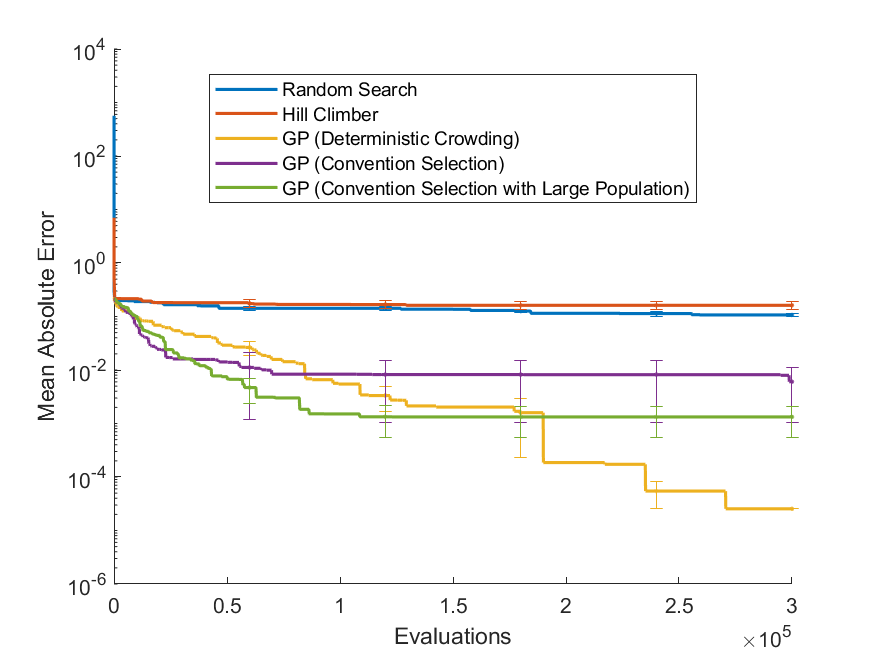
\includegraphics[width=\textwidth]{performancePlot}
	\caption[]%
	{{\small Performance Plot}}    
\end{figure}
\newpage
\subsection{Dot Plot}
\begin{figure}[H]
	\centering
	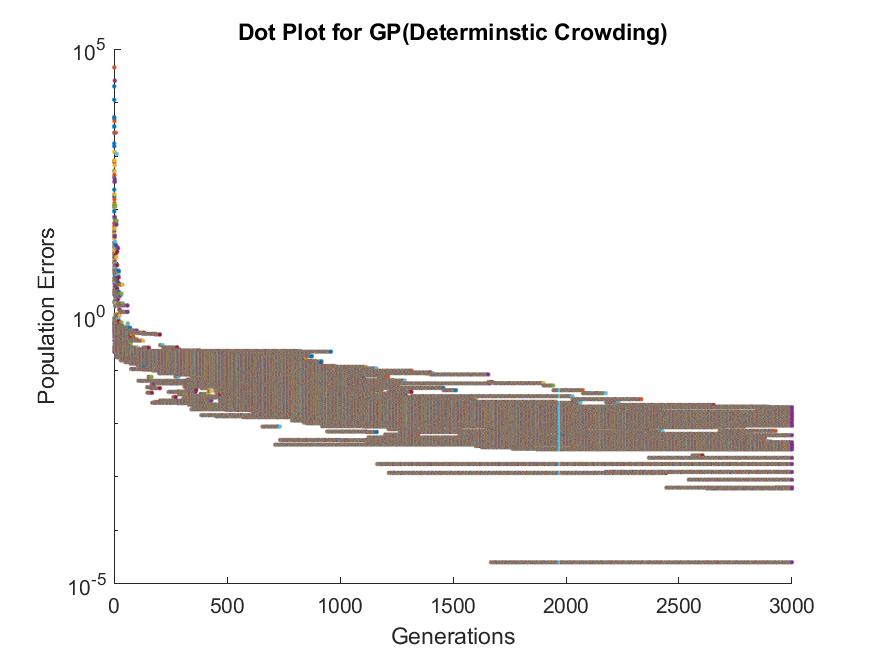
\includegraphics[width=\textwidth]{dotPlot}
	\caption[]%
	{{\small Dot Plot}}    
\end{figure}
\newpage
\subsection{Diversity Plot}
\begin{figure}[H]
	\centering
	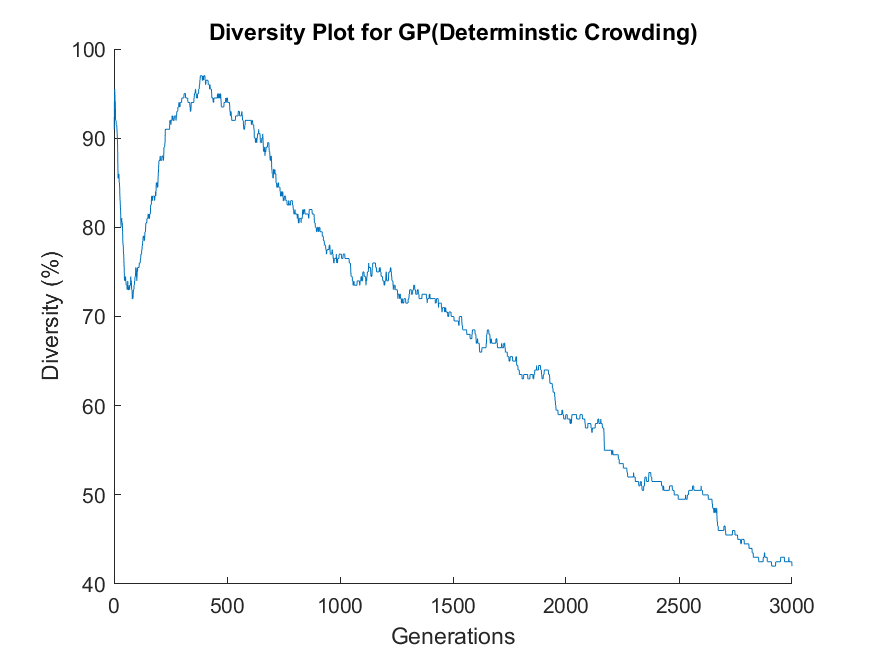
\includegraphics[width=\textwidth]{diversityPlot}
	\caption[]%
	{{\small Diversity Plot}}    
\end{figure}

\subsection{Convergence Plot}
\begin{figure}[H]
	\centering
	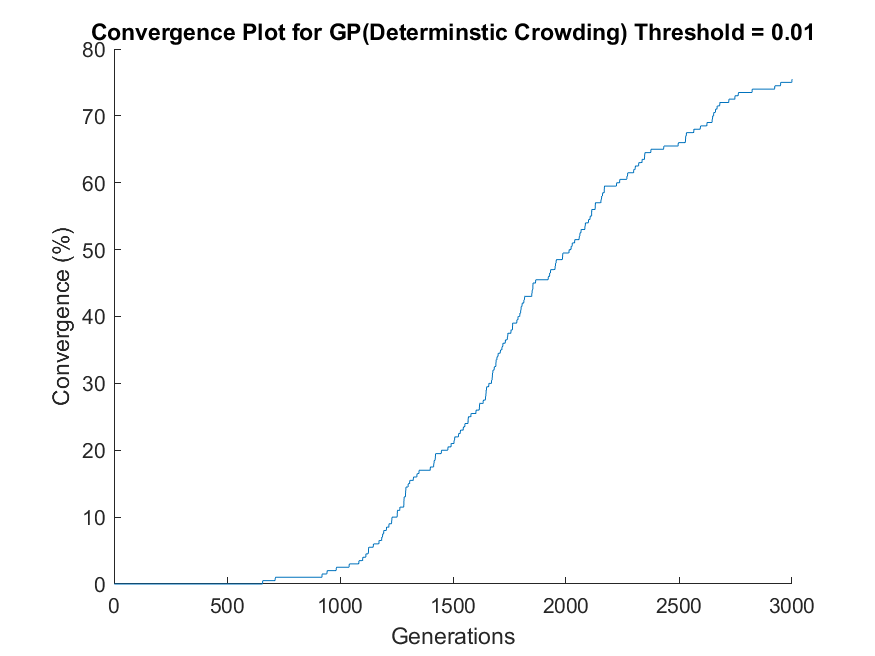
\includegraphics[width=\textwidth]{convergencePlot}
	\caption[]%
	{{\small Convergence Plot}}    
\end{figure}
\newpage
\subsection{Simpler Problem Tested}
During the debugging process of Genetic Programming, simpler problem was tested to ensure the GP can run without any bug. For example, a test data set of $sin(x)$ was used. In addition, all GPs can find the optimal solution within 10 generations.
\begin{figure}[H]
	\centering
	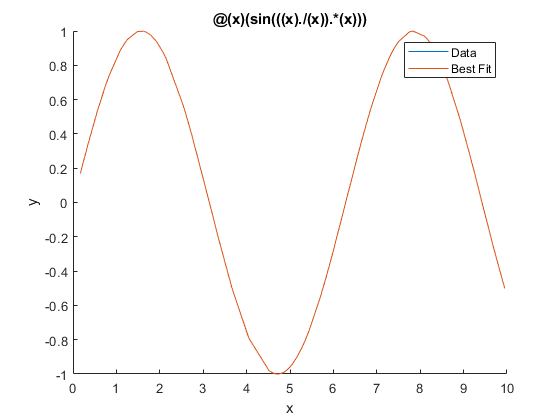
\includegraphics[width=\textwidth]{simpleProblem}
	\caption[]%
	{{\small Simple Problem Test}}    
\end{figure}

\newpage
\subsection{Validation}
The validation plot did not show much difference between training data and testing data since the data we were given has negligible noise.
\begin{figure}[H]
	\centering
	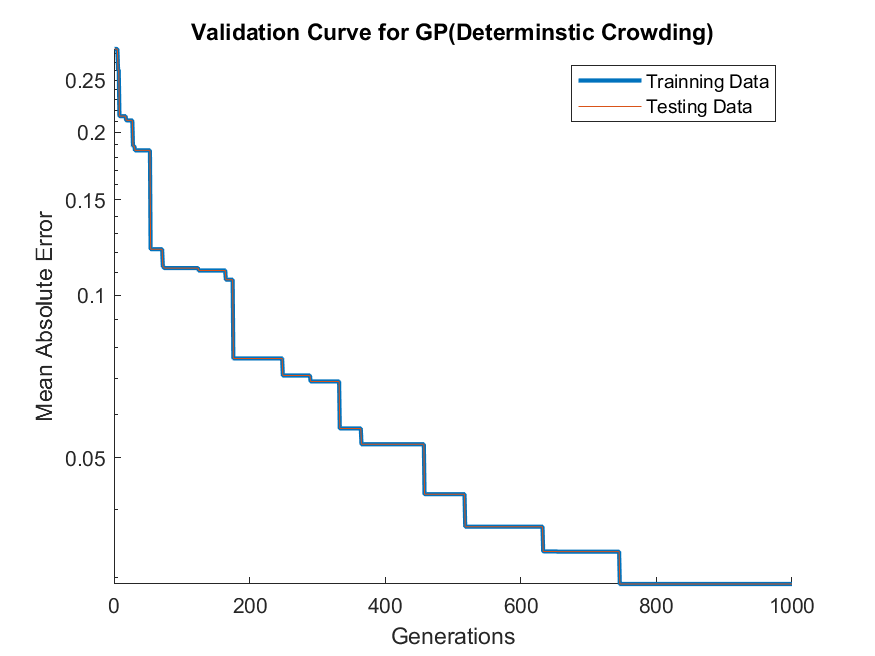
\includegraphics[width=\textwidth]{validationPlot}
	\caption[]%
	{{\small Validation Plot}}    
\end{figure}

\newpage
\section{Appendix}
\lstinputlisting{HW2.m}



\end{document}